
%%%%%%%%%%%%%%%%%%%%%%%%%%%%%%%%%%%%%%%%%%%%%%%%%%%%%%%%%%%%%%%%%%%%%%%%%%%%%%%%
\section{Estrutura da música}
\label{sec:estruturadamusica}

A música pode ser estruturada de forma modular, 
usando blocos pequenos para construir estruturas maiores.
Geralmente a estes blocos, sejam usados ou não na estrutura, se lhes atribui uma caraterística ou função;
sendo assim, existiram blocos cuja função não é requerida,
e outros que serão recorrentemente invocados;
alguns deste blocos, mesmo sendo invocados poucas vesses, 
estão colocados em pontos estratégicos, o que os convertem em indispensáveis 
para que a estrutura tenha sentido.

Uma parte importante da estruturação na composição já foi estudada na Seção \ref{sec:FormaMusical},
onde vimos distintos tipos de formas musicais, 
porem a abordagem para a criação dessas estruturas foi relativa à forma final,
sendo esta uma visão mais mecânica da composição.
Imaginemos essa abordagem, como querer armar um quebra cabeça,
percebendo só a forma das peças, tentando encaixar-lhas numa forma coerente.
Porem, nesta seção  os blocos serão ordenados, 
seguindo a função que cumprem em relação a que tipo de informação presentam ao ouvinte;
continuando a metáfora do quebra cabeça, seria equivalente a armar-lho olhando o desenho inscrito em cada bloco.
Assim, para poder abordar a composição baixo este enfoque, 
primeiro devemos descrever quais são as funções que cumprem estes blocos na música contemporânea.


%%%%%%%%%%%%%%%%%%%%%%%%%%%%%%%%%%%%%%%%%%%%%%%%%%%%%%%%%%%%%%%%%%%%%%%%%%%%%%%%
%%%%%%%%%%%%%%%%%%%%%%%%%%%%%%%%%%%%%%%%%%%%%%%%%%%%%%%%%%%%%%%%%%%%%%%%%%%%%%%%
\subsection{Partes de uma música}
\label{subsec:partesmusica}
 Podemos achar diversos tipos de blocos com que a música contemporânea é composta, 
cada um destes com distintas funções na composição musical;
assim temos:
a \hyperref[ref:Introducao]{\textbf{introdução}},
o \hyperref[ref:Verse]{\textbf{verso}},
a \hyperref[ref:Ponte]{\textbf{ponte}},
o \hyperref[ref:Coro]{\textbf{coro}},
a \hyperref[ref:Coda]{\textbf{coda}},
etc.
Nas seguintes subseções descreveremos alguns destes blocos.

%%%%%%%%%%%%%%%%%%%%%%%%%%%%%%%%%%%%%%%%%%%%%%%%%%%%%%%%%%%%%%%%%%%%%%%%%%%%%%%%
\subsubsection{Introdução}
\index{Música!Introdução}
\label{ref:Introducao}
Na música, a introdução  é uma \hyperref[ref:Secao]{\textbf{seção}} que se executa ao inicio de uma composição musical,
para anunciar ao ouvinte o ``clima'' da música. Também informa o \hyperref[sec:Andamento]{\textbf{andamento}},
 material rítmico, 
melódico e harmônico, que será usado quando inicie o corpo da composição.
Em muitas ocasiões a introdução passa a ser uma parte muito icônica de uma composição
\cite[pp. 17]{adolfo1997composicao}.

Se a composição usa vozes,  geralmente a introdução se distinguirá por só ser instrumental. 
A introdução é importante para o vocalista, pois sem esta, ele pode entrar fora do tom ou do tempo. 

%%%%%%%%%%%%%%%%%%%%%%%%%%%%%%%%%%%%%%%%%%%%%%%%%%%%%%%%%%%%%%%%%%%%%%%%%%%%%%%%
\subsubsection{Verso (Verse, Estrofe)}
\index{Música!Verse}
\index{Música!Verso}
\label{ref:Verse}
O verso é a seção inicial do corpo de uma composição musical, 
esta parte antecede à \hyperref[ref:Ponte]{\textbf{ponte}} ou ao \hyperref[ref:Coro]{\textbf{coro}}
\cite[pp. 18]{adolfo1997composicao}.
No verso é onde o compositor desenvolve a temática da composição,
e tenta passar uma mensagem, ideia ou sentimento ao ouvinte,
usando uma melodia que será usada ao longo de toda a obra, com ligeiras variações.

No primeiro verso apresentado não se joga de primeira toda a informação;
e sim, o assunto é introduzido para acordar o interesse no ouvinte,
para ser desenvolvido melhor em versos ou pontes posteriores.   

%%%%%%%%%%%%%%%%%%%%%%%%%%%%%%%%%%%%%%%%%%%%%%%%%%%%%%%%%%%%%%%%%%%%%%%%%%%%%%%%
\subsubsection{Ponte (Bridge)}
\index{Música!Ponte}
\index{Música!Bridge}
\label{ref:Ponte}

A ponte é como mínimo uma segunda seção, e procura ser contrastante com a anterior; 
a ponte prepara ao ouvinte para o retorno à tematica original expressada no verso 
\cite[pp. 18]{adolfo1997composicao}.

A ponte geralmente é usada para refletir expandindo sentimentos em relação às seções anteriores,
preparando ao ouvinte para o clímax.
Assim, a ponte é uma ótima opção para que o letrista agregue informação da história que criou nos versos.

%%%%%%%%%%%%%%%%%%%%%%%%%%%%%%%%%%%%%%%%%%%%%%%%%%%%%%%%%%%%%%%%%%%%%%%%%%%%%%%%
\subsubsection{Coro (Chorus, Refrão)}
\index{Música!Coro}
\index{Música!Chorus}
\index{Música!Refrão}
\label{ref:Coro}

é parte principal da composição, 
e geralmente  se repete muitas vezes, 
ficando como refrão na memoria do ouvinte
\cite[pp. 18]{adolfo1997composicao}.

O coro é a seção onde convergem todos os versos, 
e é onde o compositor normalmente se expressa mais emocionalmente;
sendo nesta seção onde mais se exteriorizam os estados emocionais. 
Na segunda vez que se repita o coro, 
provavelmente o compositor ache interessante incrementar ainda mais a expressividade.
A parte letrada do coro geralmente indica ou reflete sobre o título da composição.

%%%%%%%%%%%%%%%%%%%%%%%%%%%%%%%%%%%%%%%%%%%%%%%%%%%%%%%%%%%%%%%%%%%%%%%%%%%%%%%%
\subsubsection{Coda (Final, Conclusão)}
\index{Música!Coda}
\label{ref:Coda}
A coda na música é uma \hyperref[ref:Secao]{\textbf{seção}}  que é adicionada ao final de uma peça musical. 
Nesta seção podem ser usadas ou não ideais musicais já utilizadas na composição
\cite[pp. 17]{adolfo1997composicao}.



%%%%%%%%%%%%%%%%%%%%%%%%%%%%%%%%%%%%%%%%%%%%%%%%%%%%%%%%%%%%%%%%%%%%%%%%%%%%%%%%
%%%%%%%%%%%%%%%%%%%%%%%%%%%%%%%%%%%%%%%%%%%%%%%%%%%%%%%%%%%%%%%%%%%%%%%%%%%%%%%%
%\subsection{Adorno na música}

%%%%%%%%%%%%%%%%%%%%%%%%%%%%%%%%%%%%%%%%%%%%%%%%%%%%%%%%%%%%%%%%%%%%%%%%%%%%%%%%
% \subsubsection{Gancho (hook))}
% https://blog.landr.com/pt-br/como-escrever-uma-musica/

%%%%%%%%%%%%%%%%%%%%%%%%%%%%%%%%%%%%%%%%%%%%%%%%%%%%%%%%%%%%%%%%%%%%%%%%%%%%%%%%
% \subsubsection{Solo)}


%%%%%%%%%%%%%%%%%%%%%%%%%%%%%%%%%%%%%%%%%%%%%%%%%%%%%%%%%%%%%%%%%%%%%%%%%%%%%%%%
\subsection{Exemplos de composição estruturada}
\label{subsec:expartesmusica}

Seguindo as definições presentadas na Seção \ref{subsec:partesmusica},
podemos criar estruturas que nos deem um sentido de coerência na hora de compor e perceber a música;
na Figura \ref{fig:partes-musica-ex1} podemos ver algumas destas estruturas 
que estão separadas por blocos e ordenadas cronologicamente, na música, de esquerda a direita.
     \begin{figure}[!ht]
	     \centering
	     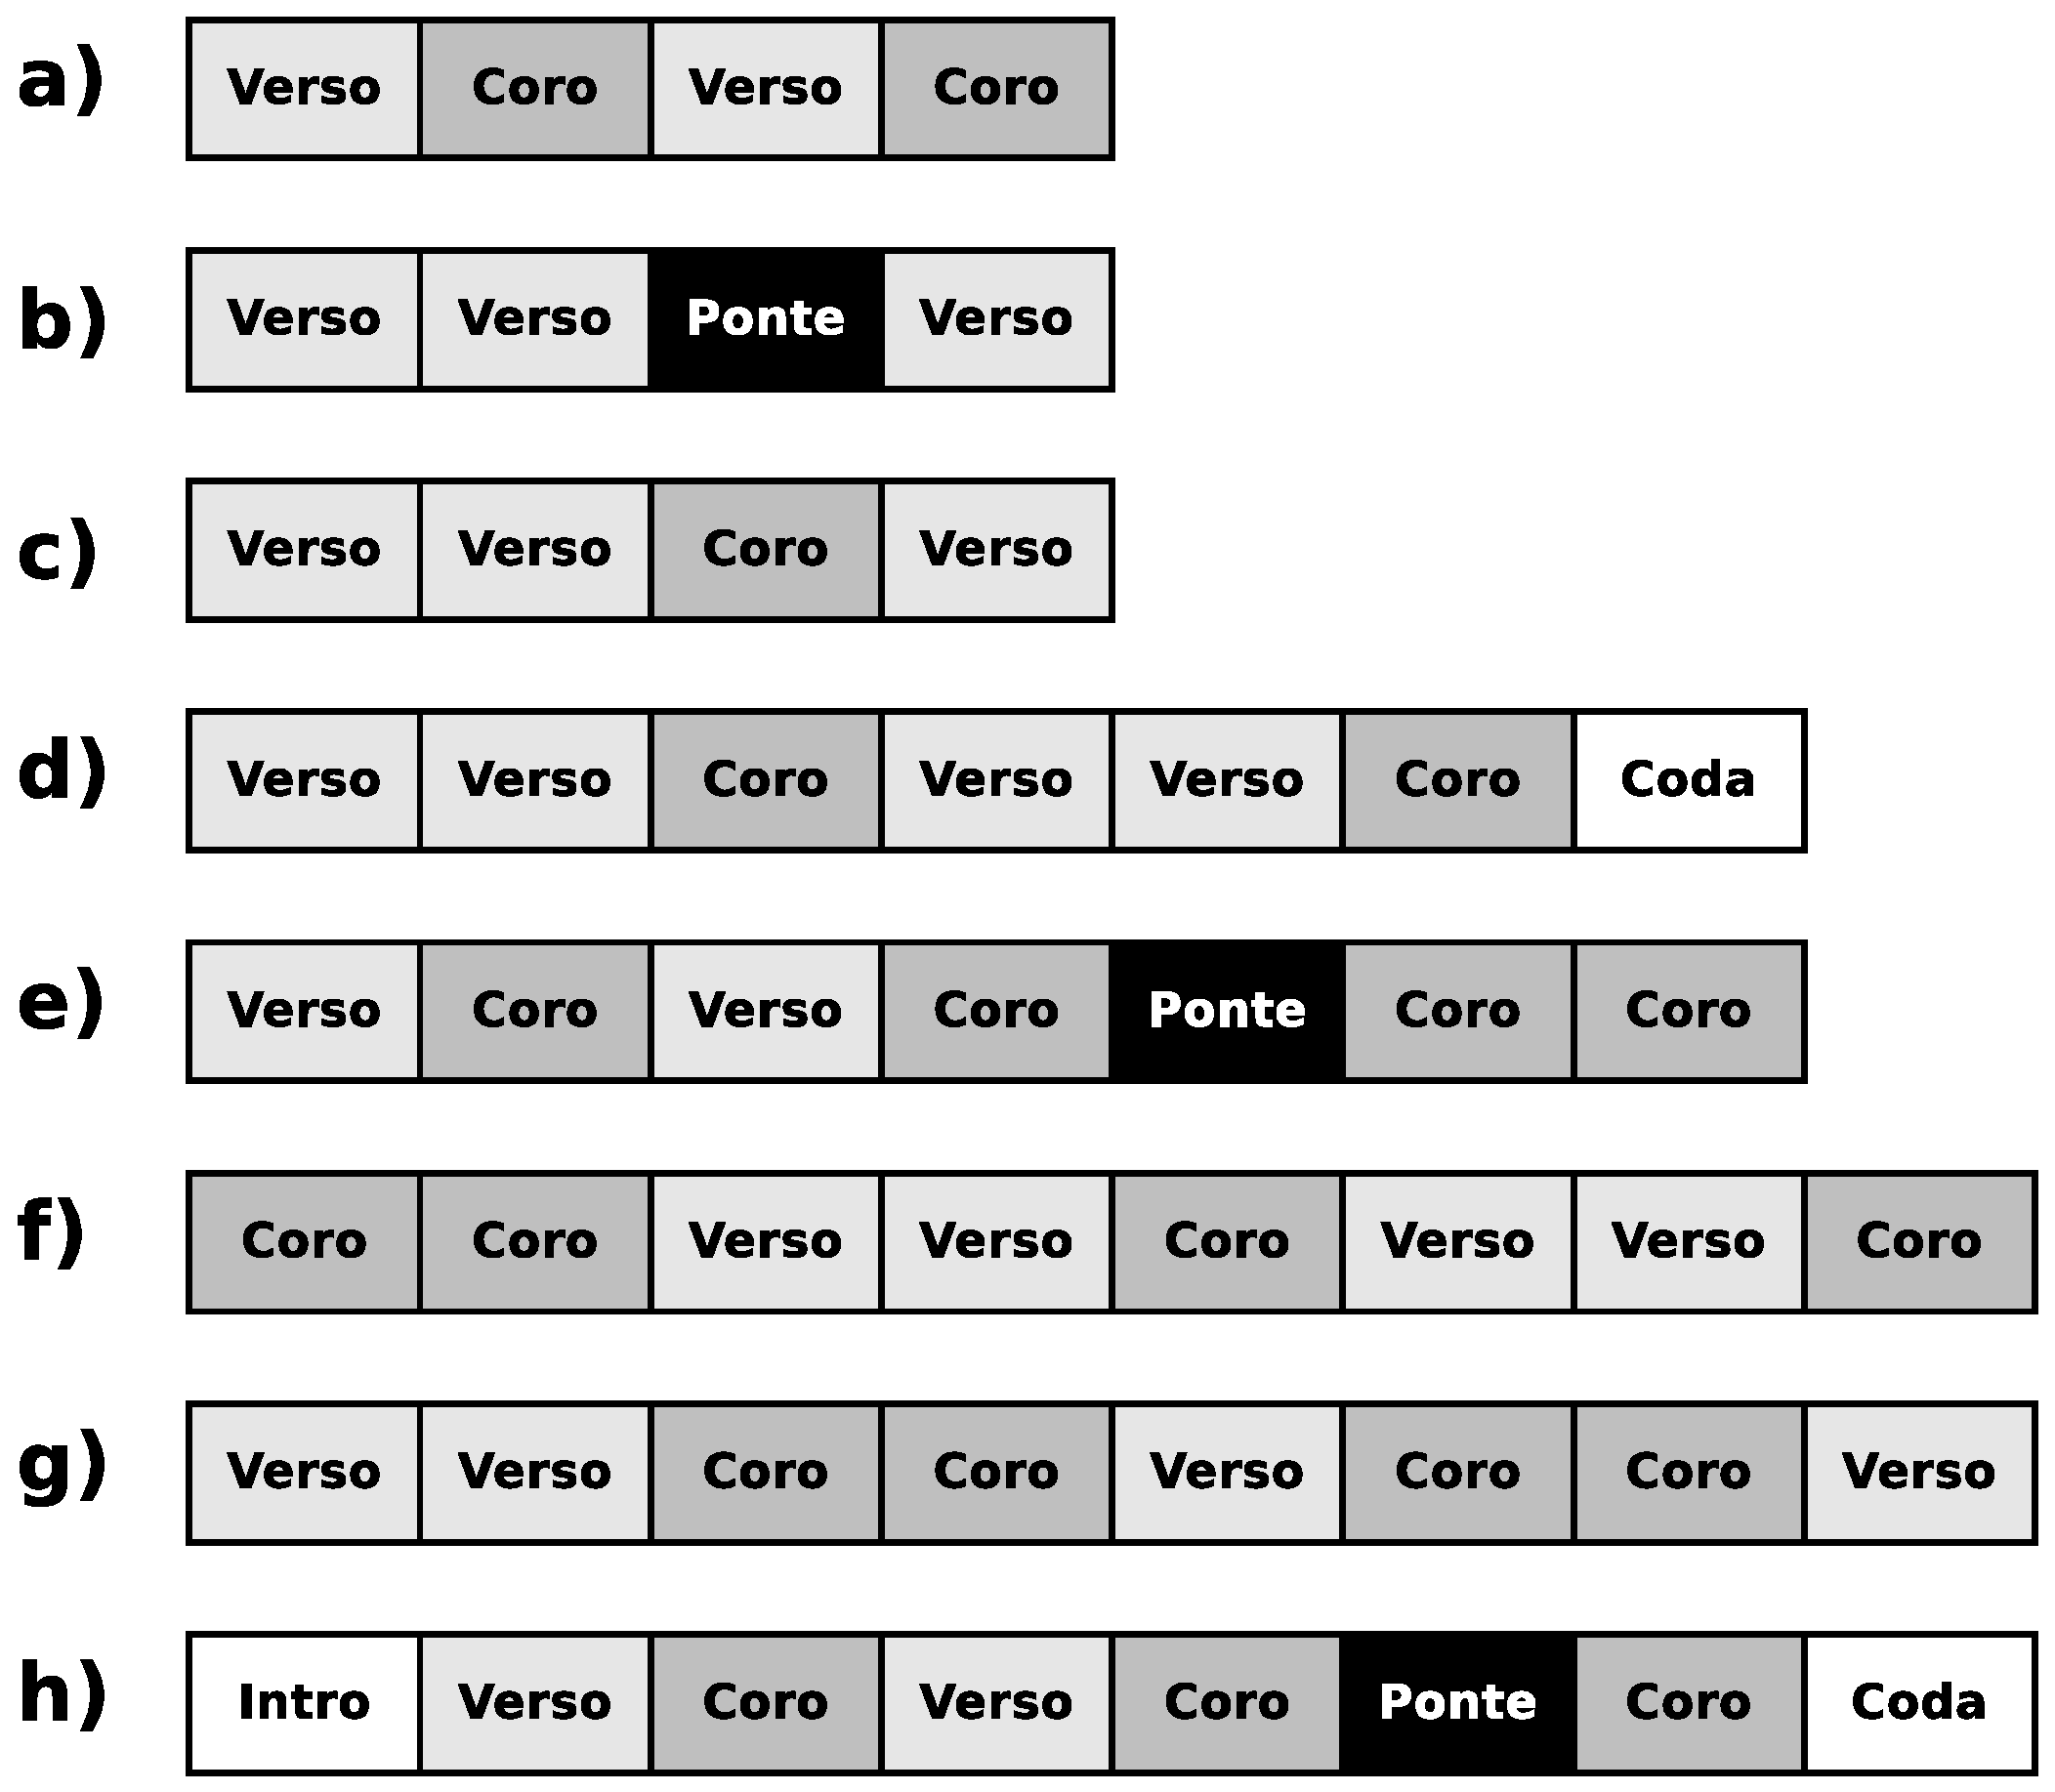
\includegraphics[width=0.75\textwidth]{chapters/cap-musica-topicos/partes-musica-ex1.eps}
	     \caption{Composisção por partes.}
	     \label{fig:partes-musica-ex1}
     \end{figure}
Assim podemos ver formas já conhecidas como:
\begin{itemize}
\item A Figura \ref{fig:partes-musica-ex1}a,
onde se usa uma \hyperref[subsec:formabinaria]{\textbf{forma binária}}.
\item Temos os casos das Figuras \ref{fig:partes-musica-ex1}b e \ref{fig:partes-musica-ex1}c,
que são \hyperref[pp. subsec:formaternaria]{\textbf{forma ternárias}}, 
especificamente na \hyperref[subsec:formacancao]{\textbf{forma canção}}. 
\item Na Figura \ref{fig:partes-musica-ex1}d temos duas formas de ver a estrutura,
como a repetição de duas formas binárias: $||:A:||B$, $||:A:||B$, 
ou como uma forma ternária seguida de uma forma binária: $||:A:||BA$, $AB$;
pertencer a uma ou outra categoria dependerá do grado de variação entre os versos e o contraste com o coro.
\item Na Figura \ref{fig:partes-musica-ex1}e temos uma forma livre.
\item Nas Figuras \ref{fig:partes-musica-ex1}f e  \ref{fig:partes-musica-ex1}g temos o uso 
da \hyperref[subsec:formarondo]{\textbf{forma rondó}} usando repetições: $||:A:||:B:||A||:C:||A$.
\item Finalmente na Figura \ref{fig:partes-musica-ex1}h temos outra forma livre.
\end{itemize}~

Em geral a qualquer das estruturas presentadas se lhe poderia agregar ou retirar o uso da introdução e da coda,
sem desmerecer a funcionalidade da estrutura.
%%%%%%%%%%%%%%%%%%%%%%%%%%%%%%%%%%%%%%%%%%%%%%%%%%%%%%%%%%%%%%%%%%%%%%%%%%%%%%%%
% http://musikinfocus.blogspot.com/2015/07/estrutura-musical.html
% http://quatertralhas.blogspot.com/2014/07/forma-uma-assim-um-samba-tom-jobim.html
% 


%%%%%%%%%%%%%%%%%%%%%%%%%%%%%%%%%%%%%%%%%%%%%%%%%%%%%%%%%%%%%%%%%%%%%%%%%%%%%%%%
%\subsection{\textbf{Composição seguindo uma estrutura narrativa}}
%\label{subsec:comonarrativa}
%% https://blog.landr.com/pt-br/como-escrever-uma-musica/


